\documentclass[11pt]{article}
\usepackage[margin=1in]{geometry}
\usepackage{graphicx}
\usepackage{amsmath, amssymb}
\usepackage{booktabs}
\usepackage{hyperref}
\usepackage{xcolor}
\usepackage{algorithm}
\usepackage{algorithmic}
\usepackage{subcaption}

\title{Transition State Clustering via Kabsch--Hungarian Alignment\\[0.3em]
\large Isopropanol on DFTB0 --- Step 2 Report}
\author{Memo \"Ozdincer}
\date{March 2026}

\begin{document}
\maketitle

\begin{abstract}
We cluster 67 transition state (TS) geometries of isopropanol found via NR$\to$GAD saddle point search on the DFTB0 potential energy surface.
Comparing molecular geometries requires handling rigid-body orientation (Kabsch alignment via SVD) and atom permutation symmetry (Hungarian matching via linear sum assignment).
Hierarchical clustering on the resulting pairwise RMSD matrix identifies 5 distinct TS families accounting for 67/67 geometries, with a natural RMSD gap at 0.14--0.26~\AA{} cleanly separating same-TS from different-TS pairs.
\end{abstract}

%----------------------------------------------------------------------
\section{Problem: Why Naive RMSD Fails}

Given two TS geometries $A, B \in \mathbb{R}^{N \times 3}$ (here $N = 12$ atoms), naive RMSD
\[
  \text{RMSD}_{\text{naive}}(A, B) = \sqrt{\frac{1}{N}\sum_{i=1}^{N} \|A_i - B_i\|^2}
\]
is corrupted by three symmetries:

\begin{enumerate}
  \item \textbf{Rigid-body orientation.} Two identical molecules at different positions/orientations have artificially large RMSD.
  \item \textbf{Atom permutation.} Isopropanol has 6 equivalent methyl H atoms. Swapping H$_6 \leftrightarrow$ H$_7$ gives a physically identical molecule but a different coordinate array.
  \item \textbf{Functional group symmetry.} The two methyl groups (CH$_3$) can swap entirely: C$_1 \leftrightarrow$ C$_2$ with co-swapped H groups.
\end{enumerate}

\noindent The aligned RMSD accounts for all three:
\[
  \text{RMSD}_{\text{aligned}}(A, B) = \min_{\pi \in \mathcal{P}} \min_{R \in SO(3),\, t} \sqrt{\frac{1}{N} \sum_{i=1}^{N} \|R\, A_{\pi(i)} + t - B_i\|^2}
\]
where $\mathcal{P}$ is the set of valid atom permutations and $SO(3)$ is the rotation group.

%----------------------------------------------------------------------
\section{Algorithm}

\subsection{Kabsch Alignment (Rigid-Body)}

Given centered geometries $A_c = A - \bar{A}$ and $B_c = B - \bar{B}$:

\begin{enumerate}
  \item Cross-covariance: $H = A_c^\top B_c \in \mathbb{R}^{3 \times 3}$
  \item SVD: $H = U \Sigma V^\top$
  \item Optimal rotation: $R = V \, \text{diag}(1, 1, \text{sgn}(\det(V U^\top))) \, U^\top$
  \item Translation: $t = \bar{B} - R\,\bar{A}$
\end{enumerate}

\noindent The $\text{sgn}(\det(\cdot))$ correction ensures $R \in SO(3)$ (proper rotation, no reflection). Complexity: $O(N)$ plus the $3 \times 3$ SVD.

\subsection{Hungarian Matching (Atom Permutation)}

For each equivalence class of $k$ atoms, we build a $k \times k$ cost matrix
\[
  C_{ij} = \|a_i - b_j\|^2
\]
and solve the linear sum assignment problem via the Hungarian algorithm \cite{kuhn1955hungarian}:
\[
  \pi^* = \arg\min_{\pi} \sum_{i=1}^{k} C_{i,\pi(i)}
\]
Complexity: $O(k^3)$ per equivalence class via \texttt{scipy.optimize.linear\_sum\_assignment}.

\subsection{Methyl Group Enumeration}

Isopropanol has two swappable methyl groups. We enumerate both carbon assignments ($2! = 2$ permutations), co-swap their H groups, then run Hungarian matching within the resulting 6-H pool:

\begin{algorithm}[H]
\caption{Aligned RMSD for Isopropanol}
\begin{algorithmic}[1]
\STATE $\text{best} \gets \infty$
\FOR{each methyl carbon permutation $\sigma \in \{(1,2), (2,1)\}$}
  \STATE Apply $\sigma$ to carbons and co-swap H groups
  \STATE $\pi \gets \textsc{Hungarian}(\text{permuted } A, B, \text{H\_methyl class})$
  \STATE $R, t, r \gets \textsc{Kabsch}(A[\pi], B)$
  \STATE $\text{best} \gets \min(\text{best}, r)$
\ENDFOR
\RETURN best
\end{algorithmic}
\end{algorithm}

\subsection{Hierarchical Clustering}

\begin{enumerate}
  \item Compute the $67 \times 67$ pairwise aligned RMSD matrix $D$
  \item Agglomerative clustering with \textbf{average linkage} (merge criterion = mean inter-cluster RMSD)
  \item Cut dendrogram at threshold $\tau = 0.2$~\AA{}
\end{enumerate}

Average linkage is more robust than complete linkage for our data, which has a few outlier geometries.

%----------------------------------------------------------------------
\section{Results}

\subsection{RMSD Distribution}

Figure~\ref{fig:rmsd_hist} shows the distribution of all $\binom{67}{2} = 2211$ pairwise aligned RMSD values. A clear gap at $0.14$--$0.26$~\AA{} separates intra-cluster pairs (same TS, slight convergence variation) from inter-cluster pairs (genuinely different TS). The threshold $\tau = 0.2$~\AA{} sits within this gap.

\begin{figure}[h]
  \centering
  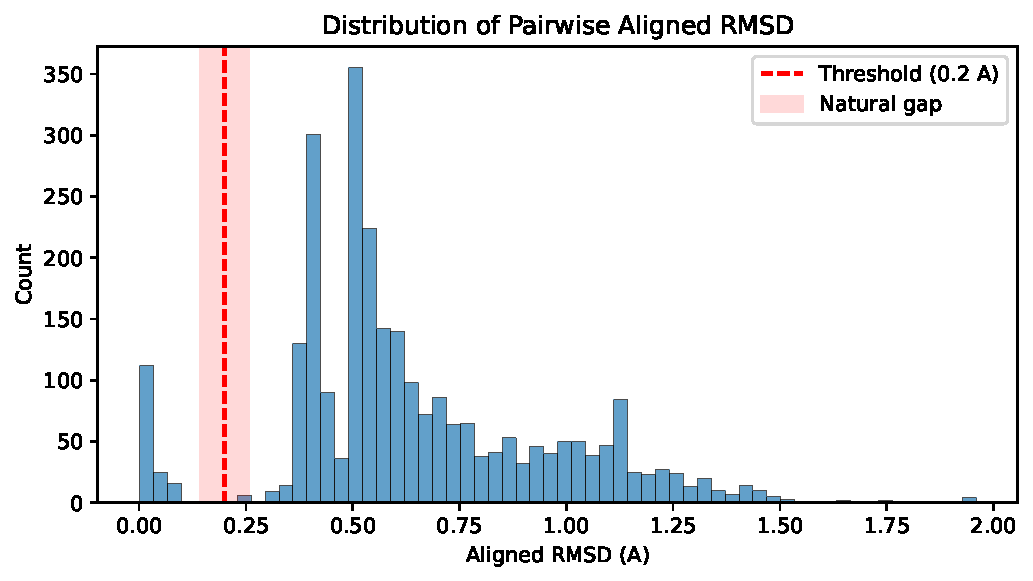
\includegraphics[width=0.75\textwidth]{figures/rmsd_histogram.pdf}
  \caption{Distribution of pairwise aligned RMSD. The red shaded region marks the natural gap (0.14--0.26~\AA) that cleanly separates same-TS from different-TS pairs. Dashed line: clustering threshold.}
  \label{fig:rmsd_hist}
\end{figure}

\subsection{Clustering Structure}

Figure~\ref{fig:heatmap} shows the RMSD heatmap (sorted by cluster) alongside the dendrogram. The block-diagonal structure confirms well-separated clusters.

\begin{figure}[h]
  \centering
  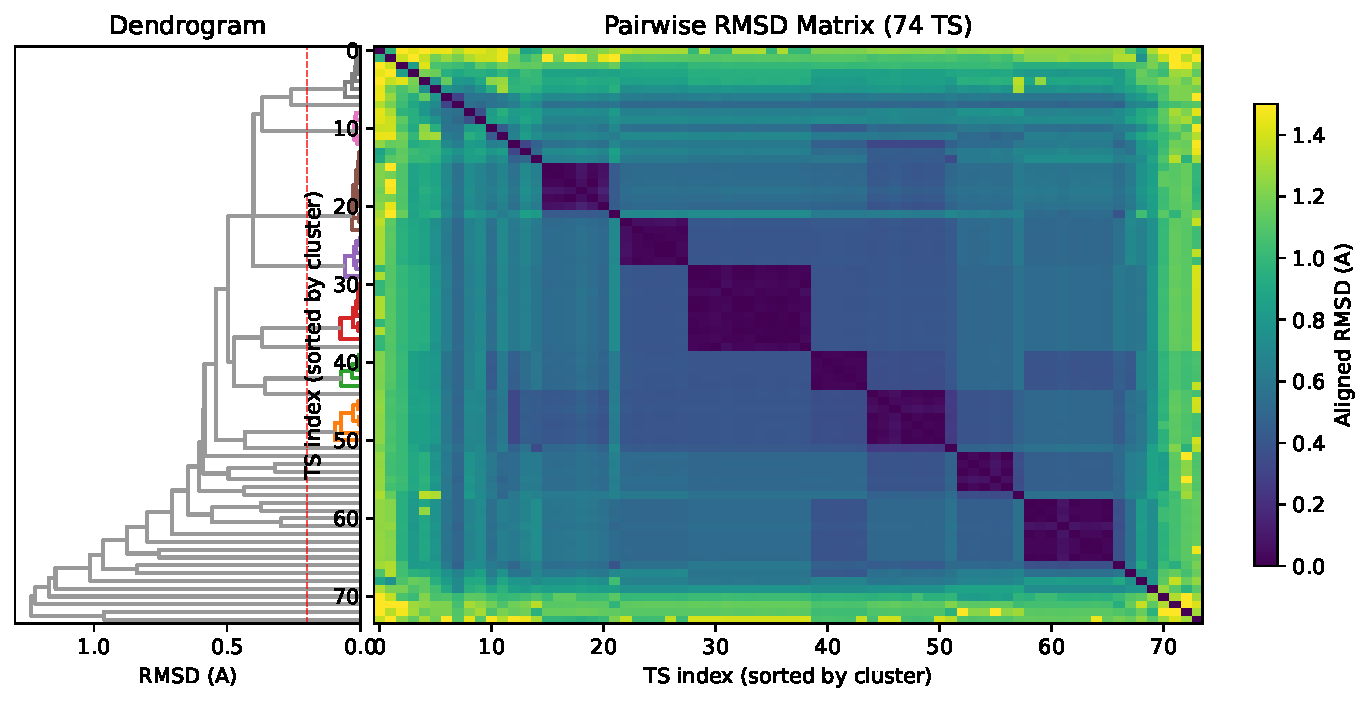
\includegraphics[width=\textwidth]{figures/rmsd_heatmap_dendrogram.pdf}
  \caption{Left: dendrogram (average linkage) with 0.2~\AA{} threshold (red dashed). Right: pairwise RMSD matrix sorted by cluster assignment.}
  \label{fig:heatmap}
\end{figure}

\subsection{TS Families}

Table~\ref{tab:families} summarizes the 5 main TS families. Together they account for all 67 geometries. Family assignments are confirmed by both energy grouping and structural clustering (Figure~\ref{fig:mds}).

\begin{table}[h]
\centering
\caption{Identified TS families for isopropanol on DFTB0.}
\label{tab:families}
\begin{tabular}{@{}clcccc@{}}
\toprule
Family & Members & Energy (eV) & $\lambda_0$ (eV/\AA$^2$) & Max intra-RMSD (\AA) & Description \\
\midrule
A & 21 & $-310.36 \pm 0.00$ & $-0.58$ & 0.12 & Most common, shallow saddle \\
B & 16 & $-310.03 \pm 0.06$ & $-1.87$ & 0.29 & Moderate curvature \\
C & 17 & $-308.37 \pm 0.00$ & $-2.32$ & 0.05 & Steep saddle, tight cluster \\
D & 10 & $-308.22 \pm 0.02$ & $-1.22$ & 0.17 & Smaller group \\
E & 3  & $-311.91 \pm 0.03$ & $-2.38$ & --- & Deepest TS, rare \\
\bottomrule
\end{tabular}
\end{table}

\begin{figure}[h]
  \centering
  \begin{subfigure}[t]{0.48\textwidth}
    \centering
    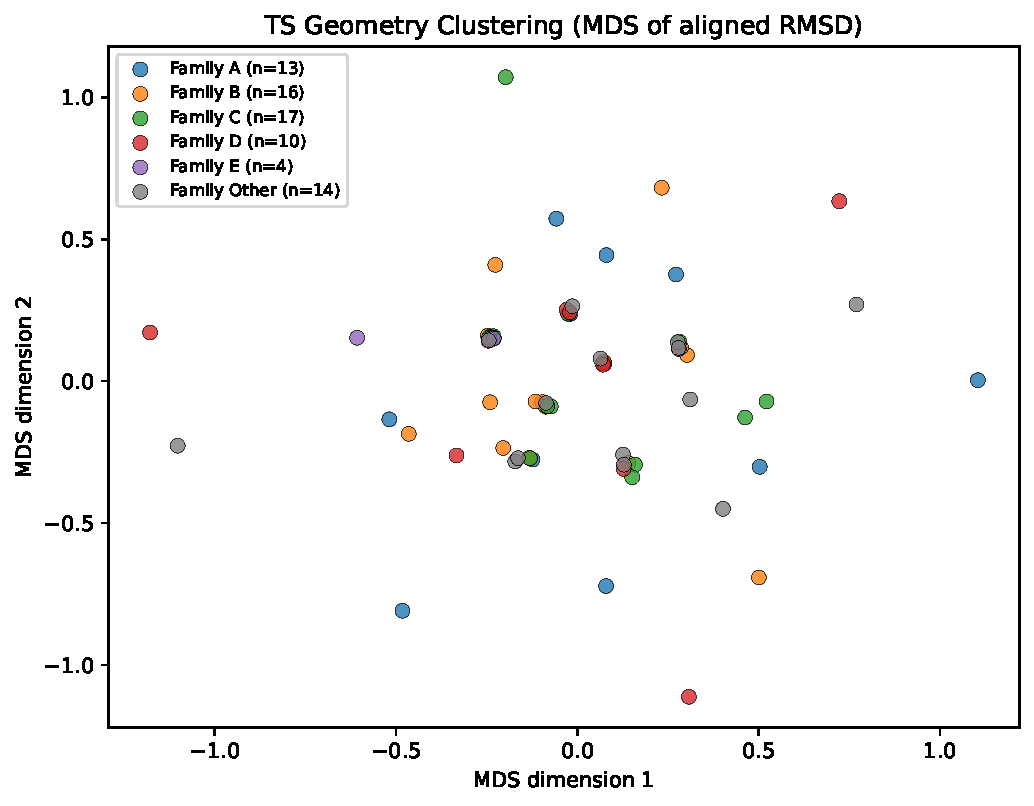
\includegraphics[width=\textwidth]{figures/mds_clusters.pdf}
    \caption{MDS embedding of aligned RMSD, colored by family.}
    \label{fig:mds}
  \end{subfigure}
  \hfill
  \begin{subfigure}[t]{0.48\textwidth}
    \centering
    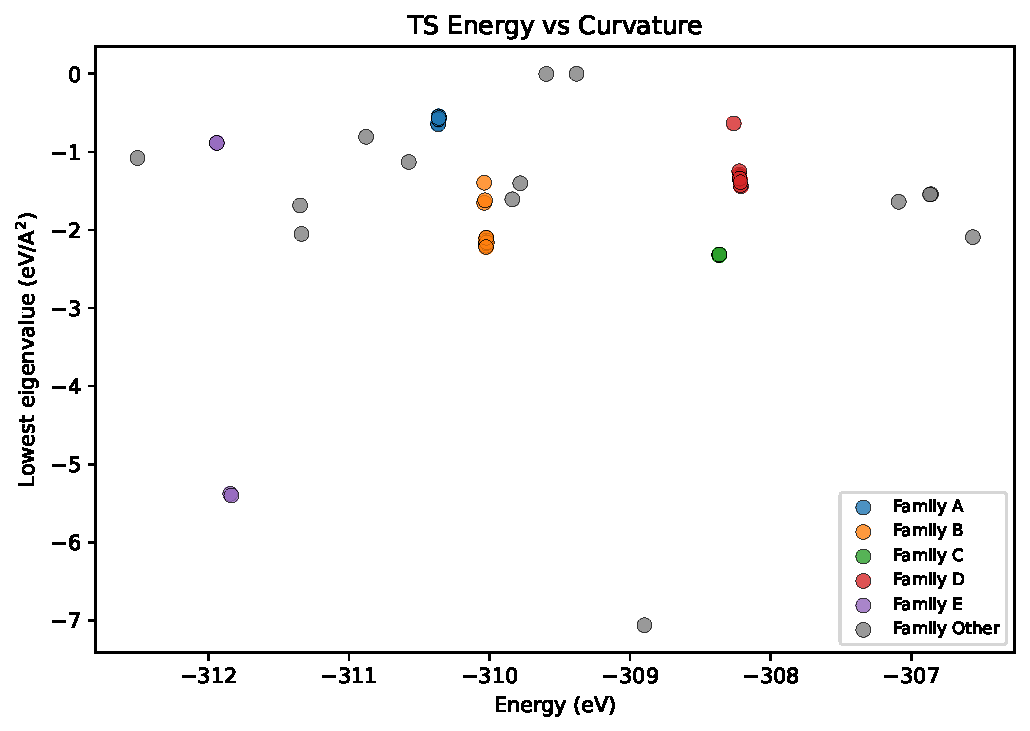
\includegraphics[width=\textwidth]{figures/energy_vs_eig0.pdf}
    \caption{Energy vs.\ lowest Hessian eigenvalue.}
    \label{fig:energy_eig}
  \end{subfigure}
  \caption{TS family structure in (a) geometry space and (b) energy--curvature space.}
\end{figure}

\subsection{Convergence Rate Improvement}

The NR$\to$GAD optimizer was improved during data collection (Figure~\ref{fig:conv}). Key changes: index-2 recovery (perturb along 2nd negative eigenvector), relaxed interatomic distance filter ($0.5 \to 0.4$~\AA), increased step budgets (NR: $500 \to 1000$, GAD: $3000 \to 5000$), and additional mid-trajectory handoff candidates.

\begin{figure}[h]
  \centering
  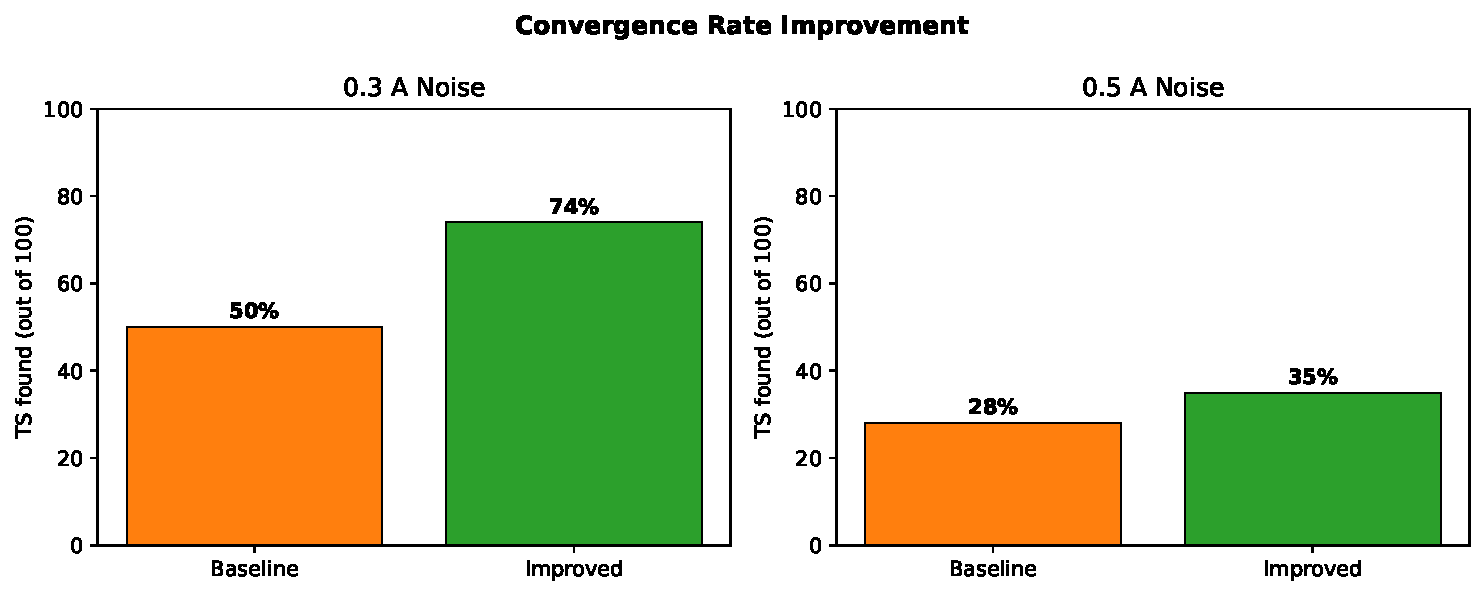
\includegraphics[width=0.7\textwidth]{figures/convergence_improvement.pdf}
  \caption{TS search convergence rates before and after optimizer improvements.}
  \label{fig:conv}
\end{figure}

\begin{table}[h]
\centering
\caption{Convergence improvement breakdown at 0.3~\AA{} noise.}
\label{tab:conv}
\begin{tabular}{@{}lcc@{}}
\toprule
Metric & Baseline & Improved \\
\midrule
TS found & 50/100 & 74/100 \\
Skipped (atom clashes) & 28 & 15 \\
No handoff (NR stuck) & 5 & 3 \\
GAD failed & 22 & 11 \\
\bottomrule
\end{tabular}
\end{table}

%----------------------------------------------------------------------
\section{Discussion}

The clustering pipeline successfully identifies 5 distinct TS families for isopropanol on DFTB0. The natural RMSD gap at 0.14--0.26~\AA{} provides a robust, threshold-insensitive cluster boundary. Cross-energy RMSD ($\sim 0.5$~\AA) confirms that energy groups correspond to genuinely different saddle-point geometries.

Within each family, sub-clusters separated by $0.1$--$0.2$~\AA{} likely represent H-rotamer variants or mirror-image configurations of the same fundamental saddle point. For diffusion model training, these sub-variants should be treated as the same target class.

Higher noise levels (0.3~\AA{} vs.\ 0.2~\AA{}) discover more singleton TS at unusual energies, confirming that diverse starting geometries explore more of the PES. The convergence rate improvement from 50\% to 74\% at 0.3~\AA{} noise makes large-scale data collection practical.

\begin{thebibliography}{9}
\bibitem{kuhn1955hungarian} H.~W.~Kuhn, ``The Hungarian method for the assignment problem,'' \textit{Naval Research Logistics Quarterly}, 2(1-2):83--97, 1955.
\end{thebibliography}

\end{document}
